\documentclass[a4paper,12pt]{article}
\usepackage[utf8]{inputenc}
\usepackage[spanish]{babel}
\usepackage{color}
\usepackage{parskip}
\usepackage{graphicx}
\usepackage{multirow}
\usepackage{listings}
\usepackage{vmargin}
\usepackage{datetime}
\newdate{date}{07}{09}{2017}
\graphicspath{ {imagenes/} }
\definecolor{mygreen}{rgb}{0,0.6,0}
\definecolor{lbcolor}{rgb}{0.9,0.9,0.9}
\usepackage{epstopdf}
\usepackage{float}


\setpapersize{A4}
\setmargins{2.5cm}       % margen izquierdo
{1.5cm}                        % margen superior
{16.5cm}                      % anchura del texto
{23.42cm}                    % altura del texto
{10pt}                           % altura de los encabezados
{1cm}                           % espacio entre el texto y los encabezados
{0pt}                             % altura del pie de página
{2cm}     

\lstset{
backgroundcolor=\color{lbcolor},
    tabsize=4,    
%   rulecolor=,
    language=[GNU]C++,
        basicstyle=\tiny,
        aboveskip={1.5\baselineskip},
        columns=fixed,
        showstringspaces=false,
        extendedchars=false,
        breaklines=true,
        prebreak = \raisebox{0ex}[0ex][0ex]{\ensuremath{\hookleftarrow}},
        frame=single,
        showtabs=false,
        showspaces=false,
        showstringspaces=false,
        identifierstyle=\ttfamily,
        keywordstyle=\color[rgb]{0,0,1},
        commentstyle=\color[rgb]{0.026,0.112,0.095},
        stringstyle=\color{red},
        numberstyle=\color[rgb]{0.205, 0.142, 0.73},
%        \lstdefinestyle{C++}{language=C++,style=numbers}’.
}


\begin{document}
\title{Final de la Primera Práctica}
\author{
Christofer Fabián Chávez Carazas \\
\small{Universidad Nacional de San Agustín de Arequipa} \\
\small{Escuela Profesional de Ciencia de la Computación} \\
\small{Computación Centrada en Redes}
}
\date{\displaydate{date}}

\maketitle

\begin{large}
 \textbf{Actividades}
\end{large}

\begin{enumerate}
 \item \textbf{Construcción del cable}
 \begin{figure}[H]
  \centering
  
\includegraphics[scale = 0.05]{1.jpg}
  \caption{Extremo del cable construido por mi.}
 \end{figure}
 \begin{figure}[H]
  \centering
  
\includegraphics[scale = 0.05]{2.jpg}
  \caption{Cable terminado}
 \end{figure}
 
 \item \textbf{Conexión usando Hyperterminal}
 \begin{figure}[H]
  \centering
  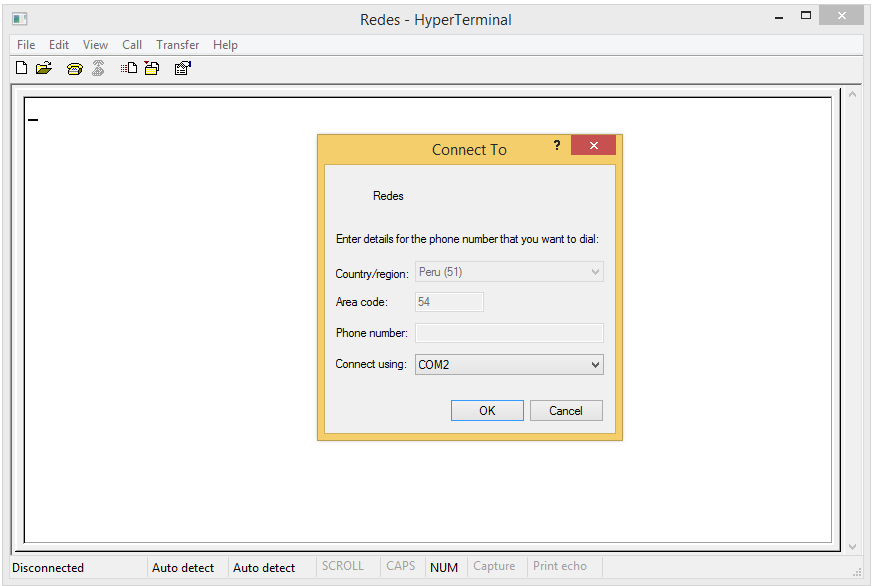
\includegraphics[scale = 0.5]{3.png}
  \caption{Configuración Hyperterminal}
 \end{figure}
 \begin{figure}[H]
  \centering
  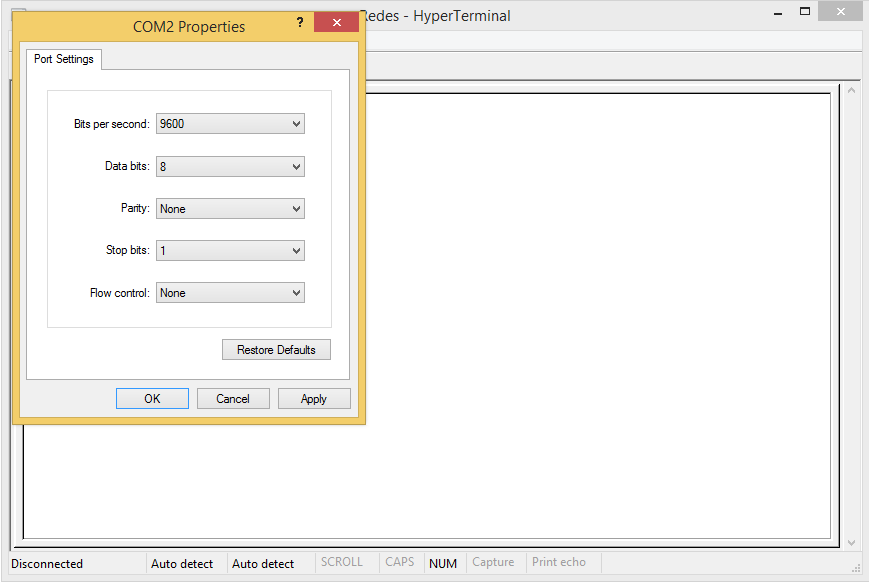
\includegraphics[scale = 0.5]{4.png}
  \caption{Configuración Hyperterminal}
 \end{figure}
 \begin{figure}[H]
  \centering
  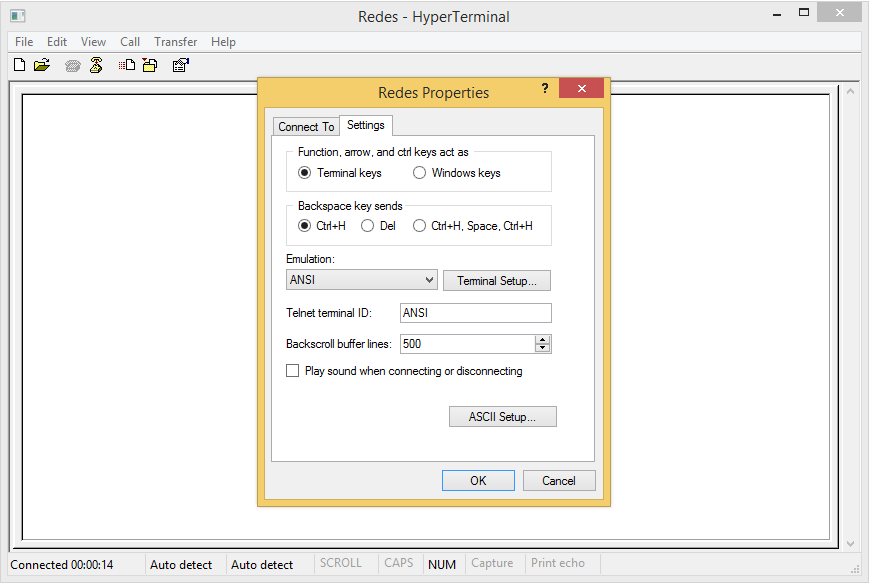
\includegraphics[scale = 0.5]{5.png}
  \caption{Configuración Hyperterminal}
 \end{figure}
 \begin{figure}[H]
  \centering
  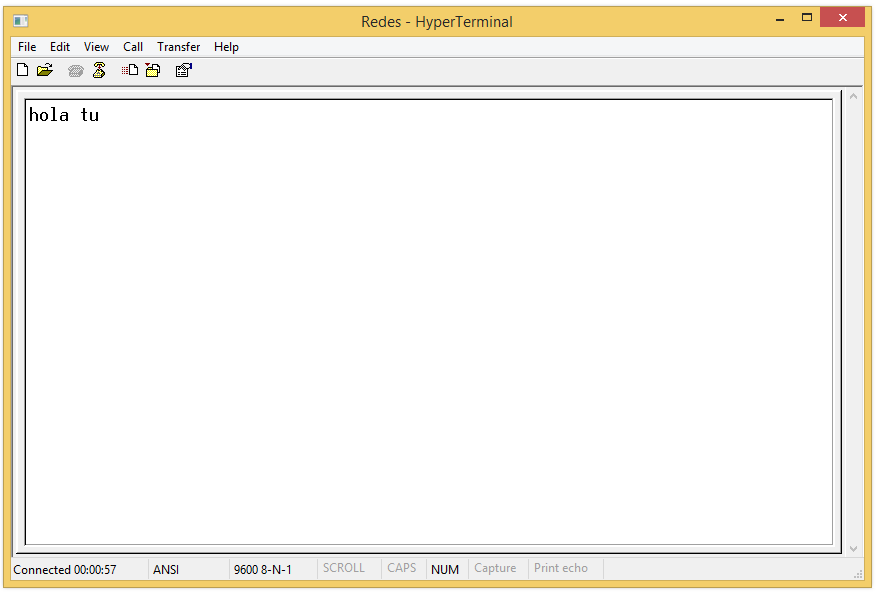
\includegraphics[scale = 0.5]{6.png}
  \caption{Comunicación en Hyperterminal}
 \end{figure}

 \item \textbf{Conexión usando ComDebug}
 \begin{figure}[H]
  \centering
  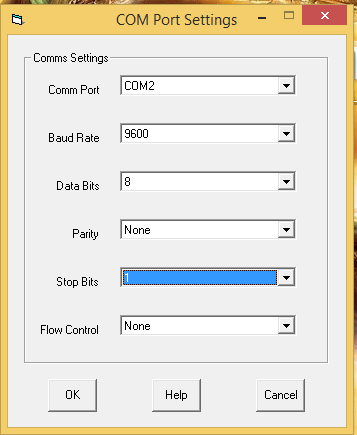
\includegraphics[scale = 0.5]{7.png}
  \caption{Configuración ComDebug}
 \end{figure}
 \begin{figure}[H]
  \centering
  
\includegraphics[scale = 0.5]{8.png}
  \caption{Comunicación en ComDebug}
 \end{figure} 
\end{enumerate}

\begin{large}
 \textbf{Cuestionario}
\end{large}


 \begin{enumerate} 
  \item \textbf{Explique el proceso de comunicación serial con control de flujo de hardware (PC a Modem)}
  
  El control de flujo es una técnica utilizada para asegurar que la entidad de transmisión no sobrecargue a la entidad receptora con una excesiva cantidad de datos.
  La entidad receptora usa una zona de memoria temporal o buffer para la transferencia. Cuando se reciben los datos, el receptor debe realizar cierta cantidad de 
  procesamiento antes de pasar los datos al software de los niveles superiores. El control de flujo por hardware utiliza líneas del puerto seria para parar o reanudar el flujo de datos y
  por lo tanto el cable de comunicaciones, además de las tres líneas fundamentales de la conexión serie: emisión, recepción y masa, ha de llevar algún hilo más para transmitir las señales de control.
  Se utilizan los niveles eléctricos reales que usa la norma serie RS-232, si esta línea está a una tensión positiva de 15 V indicará que se está en condiciones de recibir datos, y si por el contrario está a -15 V indicaría que 
  no se deben enviar más datos por el momento. El control de flujo por Hardware depende del módem para controlar el flujo de datos.
  
  \item \textbf{Busque en Internet el código de un programa confeccionado en cualquier lenguaje de programación para la comunicación serial de dos computadoras donde se utilice control de flujo por software. Destaque la parte del código donde se programe ello.}
  
  \begin{figure}[H]
   \centering
   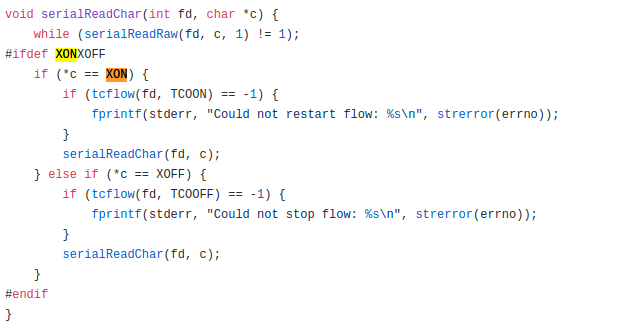
\includegraphics[scale = 0.7]{9.png}
  \end{figure}

  \item \textbf{Explique qué significan los puertos paralelo SPP, ECP y EPP y como se distribuyen los pines}
  
  \begin{itemize}
   \item \textbf{Puertos SPP (Puerto paralelo estándar)}\\
   La especificación original para el puerto paralelo era unidireccional, esto quiere decir que la información solamente puede viajar en una dirección por cada pin. Con la introducción del PS/2 en 1987, IBM ofreció un nuevo diseño de puerto paralelo bidireccional. Este modo es comúnmente conocido como puerto paralelo bidireccional, conocido como SPP (Standard Parallel Port) y ha reemplazado completamente el diseño original.
   Las comunicaciones bidireccionales permiten a cada dispositivo recibir y transmitir datos por igual. Muchos dispositivos usan los pines del 2 al 9, originalmente diseñados para el envío de datos. Pero los pines del 18 al 25, utilizados para tierra, pueden ser usados también para datos. Esto permite una comunicación full-duplex (ambas direcciones a la vez).
   \item \textbf{Puertos ECP (Puerto paralelo compatibilidad extendida)} \\
   Casi al mismo tiempo de la introducción de los puertos EPP, Microsoft y Hewlett Packard anuncian en conjunto una nueva especificación en 1992, llamada ECP (Extended Capabilities Port). Mientras que EPP estaba orientado a otros dispositivos, ECP fue diseñado para proveer una mejor funcionalidad y velocidad a las impresoras.
   En 1994, el estándar IEEE 1284 es sacado a la luz. Incluye las especificaciones EEP y ECP. Para que ambos funcionaran correctamente, tanto el sistema operativo como el dispositivo, deben soportar estos requerimientos. Hoy en día esto no suele ser un problema ya que casi todos los ordenadores soportan todos los tipos de puertos paralelos, y detectará el modo a ser usado, dependiendo el dispositivo que este conectado. Si quieres elegir un modo de forma manual, lo puedes hacer por medio de la BIOS.
   \item \textbf{Puertos EPP (Puerto paralelo mejorado)} \\
   Los puertos paralelos mejorados EPP (Enhanced Parallel Port), fueron creados en 1991 por Intel, Xircom y Zenith, y permiten la transferencia de muchos más datos por segundo. Fueron diseñados específicamente para dispositivos que no fueran impresoras que querían ser conectados al puerto paralelo, usualmente equipos de almacenamiento que necesitaban una mayor tasa de transferencia de datos.
   \begin{figure}[H]
    \centering
    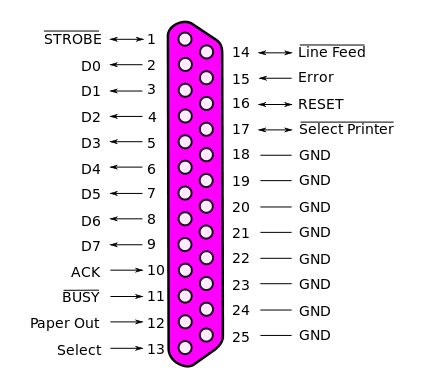
\includegraphics[scale = 0.5]{10.png}
   \end{figure}
  \end{itemize}

  \item \textbf{Defina el protocolo Kermit}
  
  Kermit es el nombre de un protocolo de transferencia y gestión de archivos, y un conjunto de programas informáticos para muchos tipos de ordenadores
  que implementan ese protocolo, así como otras funciones de comunicación que van desde la emulación de terminal a la automatización de las tareas de comunicación a través de un lenguaje de scripting de alto nivel multiplataforma. El software es independiente del transporte, operando a través de conexiones TCP/IP en el modo tradicional de texto sin cifrar, o encriptados por SSH, SSL/TLS o Kerberos IV o V, así como a través de puerto serie, módems y otros métodos de comunicación (X.25, DECnet, varios protocolos LAN como NETBIOS y LAT, puertos paralelos, etc, en determinadas plataformas).
  
  \item \textbf{¿Qué entiende por código ASCII y código ANSI?}
  
  El código ASCII es un código establecido como estándar por USA para la comunicación de datos. El código ASCII utiliza 7 bits para representar los caracteres, aunque inicialmente empleaba un bit adicional (bit de paridad) que se usaba para detectar errores en la transmisión.
  El código ANSI proviene de las siglas American National Standards Institute que es lo mismo que el código Estadounidense Estándar para el lenguaje de programación en C. 
  
  \item \textbf{Muestre la conexión de un cable Full Null Modem con DB-9 en un extremo y DB-25 en el otro.}
  
  \begin{figure}[H]
   \centering
   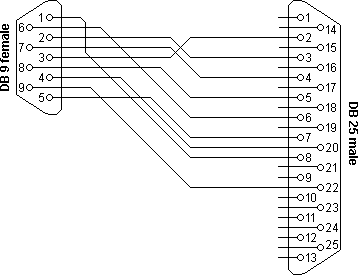
\includegraphics[scale = 0.7]{11.png}
  \end{figure}
 \end{enumerate}
  
  \begin{large}
   \textbf{Conclusiones}
  \end{large}
  
  \begin{itemize}
   \item Para la comunicación se puede utilizar Hyperterminal en un nodo y ComDebug en otro de forma normal al estar en una capa
   más arriba que el hardware.
   \item Actualmente la comunicación serial entre computadoras ya no se usa.
  \end{itemize}

  

  
 





\end{document}

